\section{Introduction}

The increase in informal settlements is a common issue faced by nations
globally.  Although informal settlements, such as slums, are commonplace in
underdeveloped countries, it affects the developed world as well, for example
refugee camps. Informal settlements might be difficult to monitor merely on the
usage of ground surveys due to the scale, distribution or a varity of other
difficulties. Remote sensing imagery provides a solution to the problems
encountered with ground based methods.  High resolution remote sensing imagery
allows for the detection of informal settlements exclusively based on features
extracted from the image.  The remote sensing imagery could conceivably be
annotated manually although the feasability diminishes with an increased scale.
As a solution, the detection of informal settlements is automated using
inherent visual characteristics of a certain area. The features extracted from remote sensing imagery provide a distinct difference between formal and
informal settlements which can be used for machine learning classification
algorithms.

\subsection{Related works and contributions}

There have been multiple studies concerning the detection of informal
settlements using remote sensing in the last decade \cite{kuffer2016slums}.
Informal settlements in the proximity of cities have been studied throughout
the globe using remote sensing imagery, e.g. Colombo \cite{colombo},
Johannesburg \cite{williams2016automatic}, Accra \cite{accra}, Mumbai
\cite{mumbai}, and Hyderabad \cite{hyderabad}. There are numerous
characteristics that are suitable to differentiate between formal and informal
settlements. This could, for example,  be the number vegetation, the width of
the roads, the size and orientations of dwellings \cite{owen2013approach}.

In general, there is a shift towards the usage of objects for the
classification of geographical features. This is broadly known as Geographic
Object-based imaga analysis or GEOBIA \cite{hay2008geographic}.Due to the
increase in availability of remote sensing high resolution imagery, it became
feasible to distinguish individual objects on a large scale.  This allows for
the interpretation of geographical imagery with individual objects at its
basis.  As a result, the characterization of regions may be based on the type
of objects that inhabit it.  To illustrate, a study classified rooftop objects
from aerial imagery of an informal settlements in Johannesburg to gather
demographic information as an alternative to traditional ground based survey
\cite{williams2016automatic}.


Our study continues partly on the work performed by Graesser et al.  A study
from 2012 conducted by Graesser et al  investigated similar
problem, the characterization of formal and informal neighborhoods.  This study
uses a collection of different features to capture the difference in
characteristics between formal and informal neighborhoods in urban
environments. Our research will evaluate if the results obtained by Graesser et
al translates well to a different city with imagery from a different
satellite. Beyond the replication of previous research, the features used by
Graesser will be extended by an additional feature. This feature will be
compared to the existing features in various measures. The features combined
will be used by a set of different classification algorithms to both assess the
performance of the feature set as well as the evaluation of various
classification algorithms.


% more detailed description of graesser paper

Graesser et al proposed a method for the detection of informal regions using
a set of different features. The features used where GLCM, HoG, Lacunarity,
LFD, LSR, NDVI, SIFT, and TEXTON. These features were calculated on satellite
image. In the processing, the paper uses blocks of pixels instead of each
individual pixel to ease the computational load. In the paper, these the size
of these blocks are 20 pixels. In our project, the block size will differ from
this for a value that works well with the features and the image data.
In addition to blocks, the paper also uses a set of different scales for the
calculation of features. A scale specifies the pixels around a block that
are used for the calculation of that block. This allows blocks to be more
spatially connected to the surrounding areas, which can increase the
performance of a feature. 


\subsection{Proposed Method}


\subsection{Data}

The image data used are captured by the earth observation satellite WorldView3
owned by DigitalGlobe. The WorldView3 satellite produces multiple categories of
imagery with varying degrees of resolution. The panchromatic images have
a resolution of 0.31 meter in contrast to  the multiband images have
a significantly lower resolution of
1.24 meter. The project uses pansharpened images, which combines the high
resolution panchromatic- and the low resolution multiband images to create
high resolution RGB images.

The content of the images contain regions of Bangalore, which is the capital
city of the indian state of Karnataka, located in south central India. The
population of the city is over ten million and is recognized as a mega city.
Banglore is known to have problems concerning informal settlements. According
to a report from 2012, there are 862 reported slums in the city


\begin{figure}
  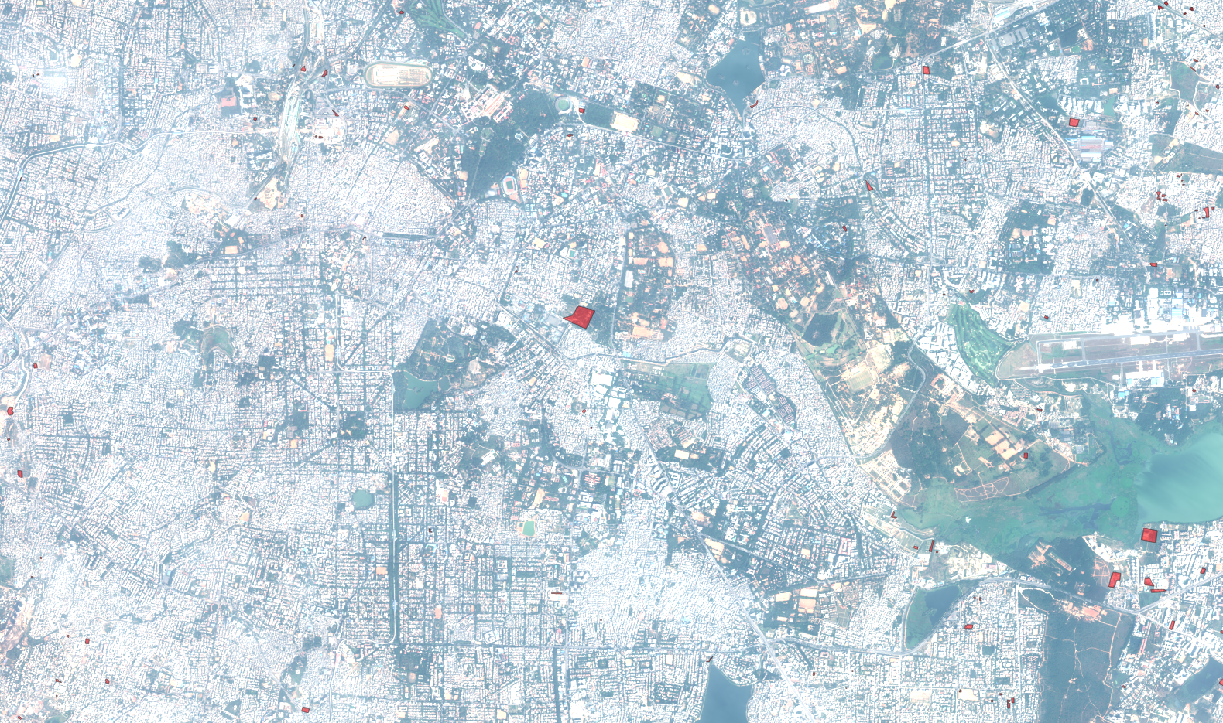
\includegraphics[width=\linewidth]{images/west-bangalore}
  \caption{A part of western Bangalore, the red patches indicate informal
  settlements}
  \label{fig:west-bangalore}
\end{figure}

\subsection{Challenges}
The distinction between formal and informal regions is often quite challenging,
in part due to the vagueness of borders between the regions. The border between
formal and informal regions often resembles more of a spectrum than a clear cut line.
Besides border difficulties, some areas are not designated as informal, while
still posessing characteristics of an informal region. This results in
a dataset with noise and inconsistency.  All in all, the binary classification
of a region encounters difficulties when applied in practice. 


Another challenge encountered in this field is the scarcity of informal
settlements.  Eventhough Banglore  has an abundance of informal settlements,
the fast majority of land is identified as formal area's. Figure
\ref{fig:west-bangalore} shows a part of western Bangalore where it is clear
that informal settlements are sparce and distributed throughout the city. As
a result, the dataset of formal and informal regions becomes quite skewed.
Furthermore, because everything that is not informal is automatically
considered formal, the formal regions have a large amount of variance of visual
properties.  To illustrate: lakes, forrests, and fields fall in the same
catagory as formal residential and industrial areas while the visual
characteristics are significantly different. The diverse content of the formal
set of visual characteristics might hinder the effectiveness of differentiating
between formal and informal regions. 

To reduce the skewedness between informal and formal, only subsections of
Figure \ref{fig:west-bangalore} are used where the proportion formal to
informal is less one-sided. The sections together with their position in the whole image, are displayed in Figure \ref{fig:sections}. A smaller difference in formal informal ratio allows for
a better understanding of the effectiveness of various features. The features
are assesed using these area's 

%\begin{figure}
%\centering
%  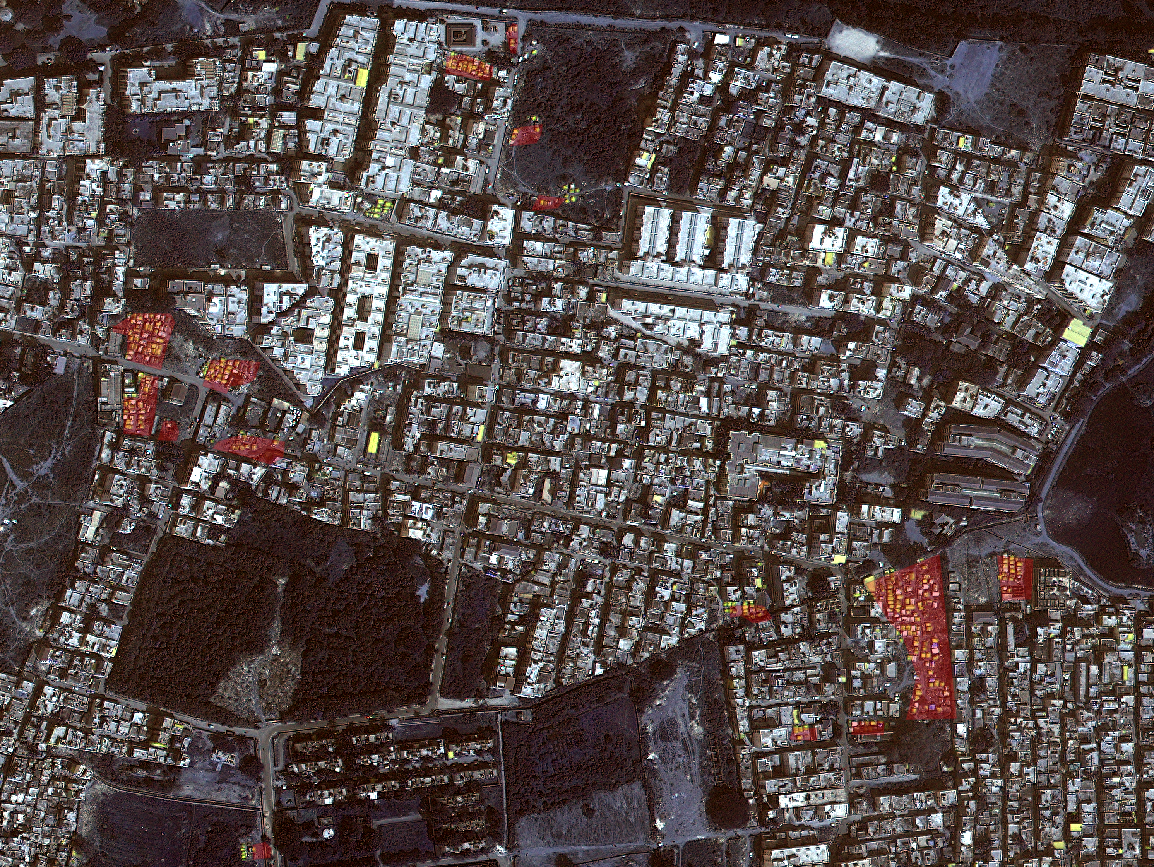
\includegraphics[width=\linewidth]{images/section_3}
%  \caption{Dense informal area in Bangalore, the red patches indicate informal
%  settlements}
%  \label{fig:section_3}
%\end{figure}


\begin{figure}
\begin{tabular}{cc}
  \subfloat[Section 1]{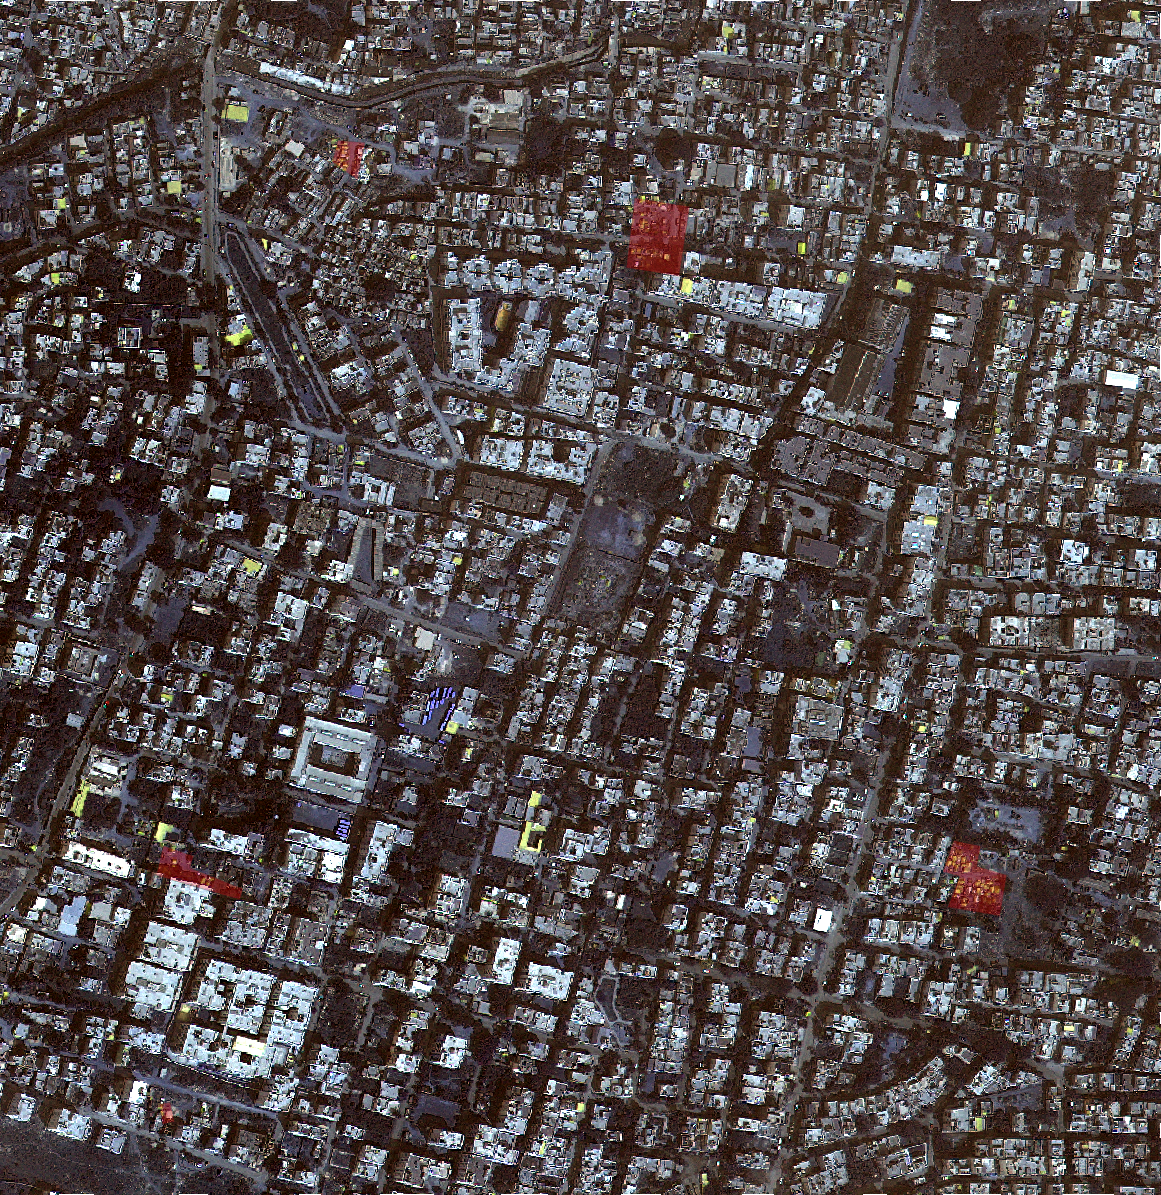
\includegraphics[width=4cm]{images/section_1}}&
  \subfloat[Section 2]{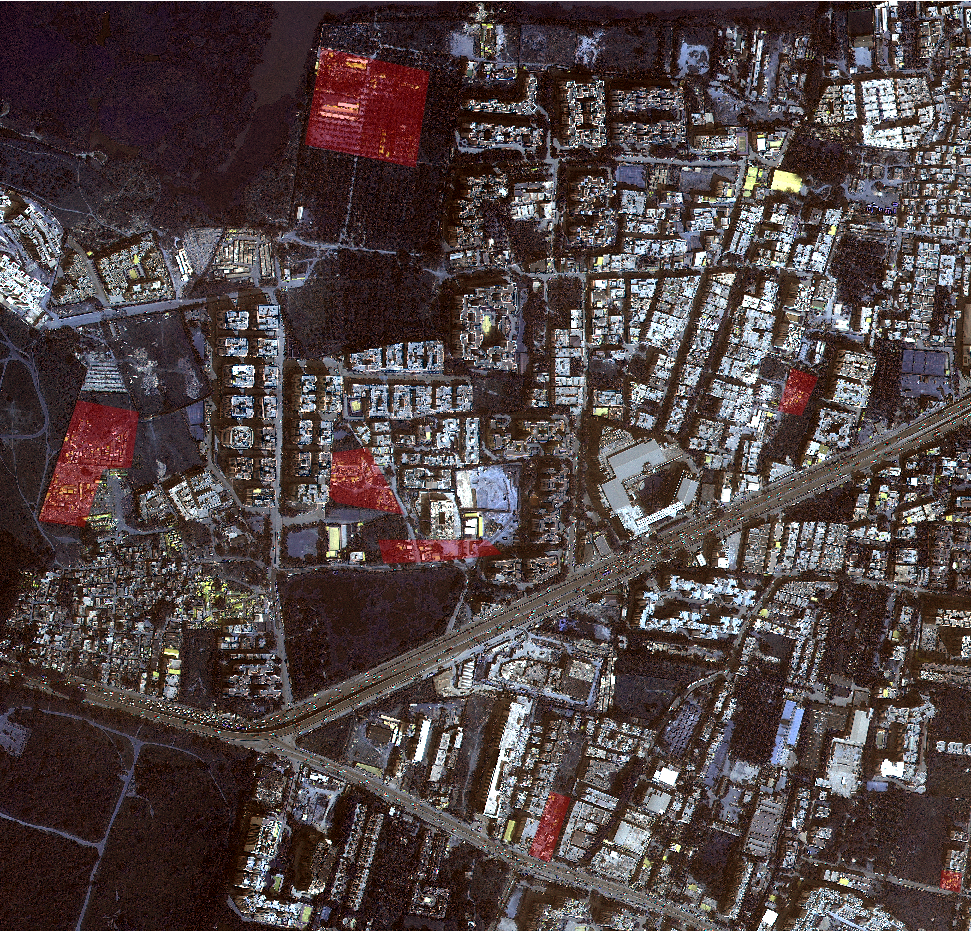
\includegraphics[width=4cm]{images/section_2}}\\
  \subfloat[Section 3]{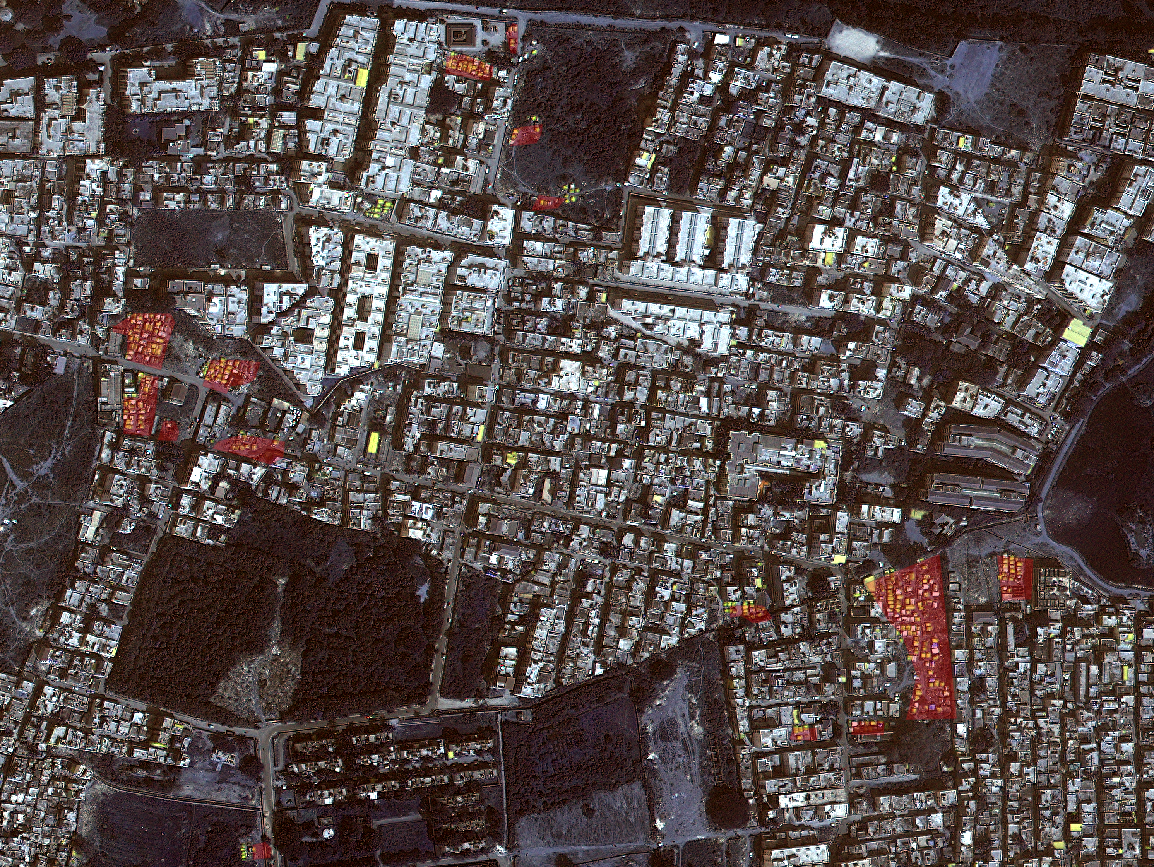
\includegraphics[width=4cm]{images/section_3}}&
  \subfloat[Location of Sections]{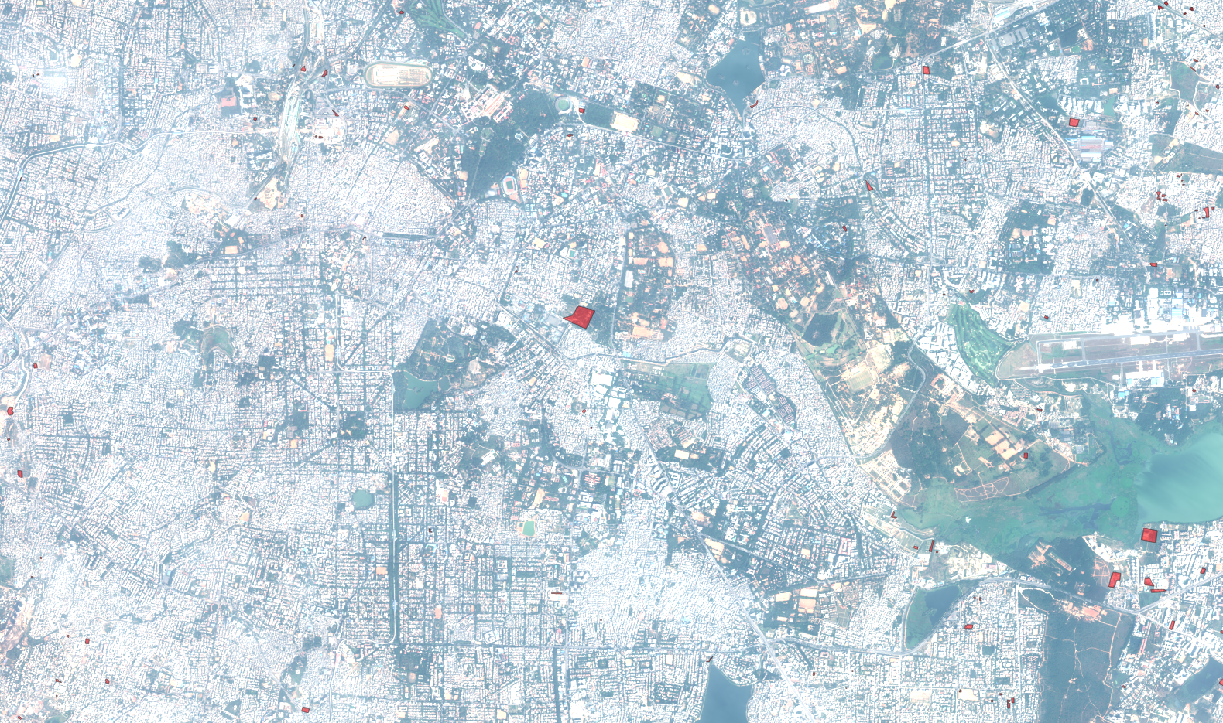
\includegraphics[width=4cm]{images/west-bangalore}}
\end{tabular}
\caption{The images used for evaluation and classification}
\label{fig:sections}
\end{figure}

